\documentclass[slidestop,usepdftitle=false,10pt]{beamer}
\usepackage[accumulated]{beamerseminar}
\usepackage[english]{babel}
\usepackage{beamertexpower}
\usepackage{multicol}
\usepackage{beamerthemeshadow}
\usepackage[ansinew]{inputenc}
\usepackage{graphics}
\usepackage{graphicx}
\usepackage{color}
\usepackage{animate}
\usepackage{bibentry}
\usepackage{epstopdf}
%\usepackage{enumerate}
\usepackage{amssymb,amsmath,graphicx,tikz,movie15}
\usepackage[linesnumbered,lined,boxed,commentsnumbered,ruled]{algorithm2e}
\usepackage{hyperref}
\usepackage[mathscr]{eucal}
\usepackage{optidef}

%\usetheme[height=0mm]{Rochester}
%\usepackage[spanish]{babel}
%\usepackage[utf8]{inputenc}
%\input adefin.tex
%\beamertemplatenavigationsymbolsempty
%\beamersetaveragebackground{white!90!red}
%**********************************************************
\newtheorem{defn}{Definition}[section]
\newtheorem{ej}{Example}[section]
\newtheorem{ejs}{Examples}[section]
\newtheorem{prop}{Proposition}[section]
\newtheorem{nota}{Notation}[section]
\newtheorem{thm}{Theorem}[section]
\newtheorem{cor}{Corollary}[section]
\newtheorem{rem}{Remark}[section]
\newtheorem{lem}{Lemma}[section]

\def \Proof{\noindent{\underline {Proof:}}}
\def\fra#1#2{\frac{ #1}{ #2}}
\renewcommand*{\baselinestretch}{1}

\def\fra#1#2{\frac{ #1}{ #2}}
%\def\fra#1#2{\frac{\displaystyle #1}{\displaystyle #2}}
%\renewcommand*{\baselinestretch}{1}

\def\fra#1#2{\frac{\displaystyle #1}{\displaystyle #2}}

%\newcommand{\fra}[2]{\displaystyle{\frac{#1}{#2}}}


\newcommand{\bi}{\mathbf{b}}
\newcommand{\ta}{\mathbf{t}}
\newcommand{\no}{\mathbf{n}}
\newcommand{\nor}{\mathbf{N}}
\newcommand{\sv}{\mathbf{S}}
\newcommand{\norm}[2]{|| #1 ||_{#2}}
\newcommand{\norma}[1]{|#1|}
\newcommand{\R}[1]{\mathbb{R}^#1}
\newcommand{\C}{\mathcal{C}^\infty}
\newcommand{\x}{\mathbf{x}}
\newcommand{\y}{\mathbf{y}}
\newcommand{\alfa}{$\alpha:(a,b)\longrightarrow\mathbb{R}^3$ }
\newcommand{\dom}{\text{dom }}
\newcommand{\Pl}{\CMcal P_l}
\newcommand{\Dl}{\CMcal D_l}

%%%%%%%%%%%%%%%%%
\definecolor{31}{rgb}{.3,.5,.2}
\definecolor{13}{rgb}{.1,.6,.3}
% CHANGED: Moved \title and \author outside of slide
\title[Coordinated and Non-Coordinated Routing Problems with Drones]{\textsc{Coordinated and Non-Coordinated Routing Problems with Drones}}
\author[Congreso Fuengirola 2021]{Carlos Valverde Mart\'in}
\newline
\institute{
	\begin{center}
		\date{}
		\text{Congreso Fuengirola 2021}
	\end{center}
	\begin{center}
		\textcolor{blue}{Joint work with Justo Puerto Albandoz}
	\end{center}
	\begin{center}
		
\includegraphics[width=0.25\textwidth]{logo.jpg}
	\end{center}
}
\date{}
\begin{document}
	\begin{frame}
		\titlepage
	\end{frame}
	%Trasparencias
	
	\begin{frame}
		\frametitle{Contents}
		\begin{enumerate}
			\item Motivation for the use of drones
			
			\item Non-Coordinated Models
			\begin{enumerate}
				\item The Crossing Postman Problem with Neighborhoods (XPPN)
			\end{enumerate}
			\item Coordinated Models
			\begin{enumerate}
				\item The mothership and drone routing problem with Graphs (MDRPG)
				% \begin{itemize}
				% 	\item Description of the Problem
				% 	\item 
				% \end{itemize}
				\item The all-terrain mothership and multiple drone routing problem with Graphs (AMMDRPG)
			\end{enumerate}
			\item Further research
		\end{enumerate}
	\end{frame}

	\section{Non-Coordinated Models: XPPN}
	\begin{frame}{Contents}
	    \begin{itemize}
		    \item Description of the Problem
		    \item Formulations
		    \item Example
		    \item Heuristic
		    \item Strenghtening results for the formulation
		    \item Benders decomposition
		    \item Computational Experiments
		\end{itemize}
	\end{frame}
	\begin{frame}
		\frametitle{Description of the Problem}
		\begin{itemize}
			\item Our problem (XPPN) combines the Crossing Postman Problem (XPP) and Travelling Salesman Problem with Neighborhoods (TSPN). 
			\item The XPP was worked by Garfinkel in \cite{garfinkel1999crossings}. It is a relaxation of the Rural Postman Problem because it is permitted to leave the edges of the network and cross from one to another at points other than the original vertices.
			\item The TSPN (see \cite{TSPN}) is a extension of the TSP because points are replaced by neighborhoods (that we assume to be convex).
			\item It is also related to the Minimum Spanning Tree with Neighborhoods (MSTN) whose details can be found in Blanco, Fernandez, Puerto \cite{MSTN}.
			\item This work can be applied to Routing Problems with Umanned Aerial Vehicles because their movement are not limited.
		\end{itemize}
	\end{frame}
	
	\begin{frame}{Description of the Problem}
    We have two nature of sets where the points can be located:
    \bigskip
    \begin{itemize}
        \item Second Order Cone representable sets:
        \begin{tiny}
        \begin{equation}\label{U-C}\tag{$\mathcal U$-C}
             x_v^i\in \mathcal U_v \Longleftrightarrow
             \left\{
             \begin{array}{cclr}
              \|A_v^{j_\ell} x_v^i + b_v^{j_\ell}\|& \leq & (c_v^{j_\ell})^T x_v^i + d_v^{j_\ell}+ M_v^{j_\ell}(1-\chi_v^{i\ell}), & \ell=1,\ldots,m_v, j_\ell=1,\ldots,n_{\ell v}, \\
             \sum_{\ell = 1}^{m_v} \chi_v^{i\ell}  & =    & 1.
             \end{array}
             \right.
        \end{equation}
        \end{tiny}
        \item Polygonal Chains where we have to cross a percentage $\alpha$ of its total length:
        \begin{tiny}
        \begin{equation}\label{P-C}\tag{$\mathcal P$-C}
             x_v^i\in \mathcal P_v \Longleftrightarrow
             \left\{
             \begin{array}{cclr}
              \lambda_v^i - j                    & \geq & \gamma_v^{ij} - (n_{Sv}+1)(1-\mu_v^{ij}),                            & j=2,\ldots,n_{Sv}+1 \\
              \lambda_v^i - j                    & \leq & \gamma_v^{ij} + (n_{Sv}+1)(1-\mu_v^{ij}),                            & j=2,\ldots,n_{Sv}+1 \\
              \gamma_v^{i1}                      & \leq & \mu_v^{i1} & \\
              \gamma_v^{ij}                      & \leq & \mu_v^{ij-1} + \mu_v^{ij}                                         & j=2,\ldots,n_{Sv}\\
              \gamma_v^{in_{Sv}}                    & \leq & \mu_v^{in_{Sv}} \\
              \sum_{j = 1}^{n_{Sv}} \mu_v^{ij}      & =    & 1 \\
              \sum_{j = 1}^{n_{Sv}+1} \gamma_v^{ij} & =    & 1 \\
              x_v^i                              & = & \sum_{j=1}^{n_{Sv}+1}\gamma_v^{ij}A_v^j \\
             \end{array}
             \right.
        \end{equation}
        \begin{equation}\label{alpha-C}\tag{$\alpha$-C}
             |\lambda_v^1-\lambda_v^2|\geq \alpha_v n_{Sv} \Longleftrightarrow
             \left\{
             \begin{array}{ccl}
              \lambda_v^1 - \lambda_v^2                       & =    & \lambda^{\text{max}}_v - \lambda^{\text{min}}_v \\
              \lambda^{\text{max}}_v + \lambda^{\text{min}}_v & \geq & \alpha_v n_{Sv}                                    \\
              \lambda^{\text{max}}_v                          & \leq & n_{Sv}(1-u_v)                                      \\
              \lambda^{\text{min}}_v                          & \leq & n_{Sv} u_v.                                       \\
             \end{array}
             \right.
        \end{equation}
        \end{tiny}
    \end{itemize}
	\end{frame}
	
	\begin{frame}{Formulations}
	    We present alternative MINLP formulations for the XPPN:
	    \begin{itemize}
	        \item Time dependent formulation. The idea is to make variables dependent on the index of the stage when an element is visited in the sequence of visited elements.
	        \footnotesize
	        \begin{mini!}|s|
            {}{\sum_{t=1}^{|V|}\sum_{v\neq w} d_{vw}^tz_{vw}^t+\sum_{t=1}^{|V|}\sum_{v\in V}f_v^t d_v^t\label{eq:obj_fun_time}}{}{}
            \addConstraint{d_{vw}^t}{\geq \beta_{vw}^t \|x_v^2 - x_w^1\|,}{\qquad\forall v\neq w}
            \addConstraint{d_v^t}{\geq \beta_{v}^t \|x_v^1 - x_v^2\|,}{\qquad\forall v\in V}
            \addConstraint{\sum_{v\in V}y_v^t}{= 1, \label{eq:connectivity1a}}{\qquad\forall t}
            \addConstraint{\sum_{t=1}^{|V|}y_v^t}{= 1, \label{eq:connectivity1b}}{\qquad\forall v\in V}
            \addConstraint{y_v^t + y_{w}^{t+1}-1}{\leq z_{vw}^t, \label{eq:subtour1}}{\qquad\forall e=(v, w)\in E_{\text{out}},\,t=1,\ldots,|\mathcal C|-1}
            \addConstraint{\eqref{U-C}, \eqref{P-C}, \eqref{alpha-C} \label{domain}}{}{}
            %\addConstraint{|\lambda_v^1 - \lambda_v^2|}{\geq \alpha_v,}{\qquad\forall v\in V_\mathcal P}
            %\addConstraint{x_v^i}{\in \mathcal P_v}{\qquad\forall v\in V_\mathcal P,\,i=1,2}
            %\addConstraint{\|B_vx_v^i+b_v\|}{\leq c_v^Tx_v^i + u_v,}{\qquad\forall v\in V_\mathcal C,\,i=1,2}
            \end{mini!}
	    \end{itemize}
	\end{frame}
	
	\begin{frame}{Formulations}
	    We present alternative MINLP formulations for the XPPN:
	    \begin{itemize}
	        \item Non-time dependent formulations. % The idea is to simplify this formulation making it independent of time at the price of losing some of its time-dependent characteristics.
	        \scriptsize
            \begin{mini*}|s|
             {}{P = \sum_{e\in E_\text{out}} p_e + \sum_{v\in V} f_v d_v}{}{}\label{SEC-XPPN}\tag{SEC-XPPN}
            \addConstraint{p_e}{\geq d_e - M_e(1 - z_e)\quad}{\forall e\in E_\text{out}}{}\tag{LIN-Mc}
            \addConstraint{p_e}{\geq m_e z_e\quad}{\forall e\in E_\text{out}}{}\label{VI-1}\tag{VI-1}
            \addConstraint{d_v}{\leq M_v\quad}{\forall v\in V}{}\label{VI-2}\tag{VI-2}
            % \addConstraint{z\in\mathcal T_{G}}{}
             \addConstraint{\sum_{w\in V\setminus\{v\}} z_{vw}}{=1,\quad}{\forall v \in V}{}\label{C1}\tag{C$_1$}
             \addConstraint{\sum_{w\in V\setminus\{v\}} z_{wv}}{=1,\quad}{\forall v \in V}{}
             \label{C2}\tag{C$_2$}
             \addConstraint{\sum_{e=(v, w):v,w\in S} z_e}{\leq |S| - 1,\quad}{\forall S\CV{\subsetneq} V}{}\label{SEC}\tag{SEC}
            \addConstraint{d_e}{\geq \|x_v^1-x_w^2\|_2\quad}{\forall e = (v, w) \in E_\text{out}}{}\label{D1}\tag{D$_1$}
            \addConstraint{d_v}{\geq \|x_v^1-x_v^2\|_2\quad}{\forall v \in V}{}\tag{D$_2$}
            \addConstraint{\eqref{U-C}, \eqref{P-C}, \eqref{alpha-C}}{}{}
            \end{mini*}
	    \end{itemize}
	\end{frame}
	
	\begin{frame}{Formulations}
	    We present alternative MINLP formulations for the XPPN:
	    \begin{itemize}
	        \item Non-time dependent formulations. % The idea is to simplify this formulation making it independent of time at the price of losing some of its time-dependent characteristics.
	        \scriptsize
            \begin{mini*}|s|
             {}{P = \sum_{e\in E_\text{out}} p_e + \sum_{v\in V} f_v d_v}{}{}\label{SEC-XPPN}\tag{sSEC-XPPN}
            \addConstraint{p_e}{\geq d_e - M_e(1 - z_e)\quad}{\forall e\in E_\text{out}}{}\tag{LIN-Mc}
            \addConstraint{p_e}{\geq m_e z_e\quad}{\forall e\in E_\text{out}}{}\label{VI-1}\tag{VI-1}
            \addConstraint{d_v}{\leq M_v\quad}{\forall v\in V}{}\label{VI-2}\tag{VI-2}
            % \addConstraint{z\in\mathcal T_{G}}{}
             \addConstraint{\sum_{w\in V\setminus\{v\}} z_{vw}}{=2,\quad}{\forall v \in V}{}
             \addConstraint{\sum_{e=(v, w):v,w\in S} z_e}{\leq |S| - 1,\quad}{\forall S\CV{\subsetneq} V}{}\label{SEC}\tag{SEC}
            \addConstraint{d_e}{\geq \|x_v^1-x_w^2\|_2\quad}{\forall e = (u, v) \in E_\text{out}}{}\label{D1}\tag{D$_1$}
            \addConstraint{d_v}{\geq \|x_v^1-x_v^2\|_2\quad}{\forall v \in V}{}\tag{D$_2$}
            \addConstraint{\eqref{U-C}, \eqref{P-C}, \eqref{alpha-C}}{}{}
            \end{mini*}
	    \end{itemize}
	\end{frame}
	
	\begin{frame}{Formulations}
	    We present alternative MINLP formulations for the XPPN:
	    \begin{itemize}
	        \item Non-time dependent formulations. % The idea is to simplify this formulation making it independent of time at the price of losing some of its time-dependent characteristics.
	        \scriptsize
            \begin{mini*}|s|
             {}{P = \sum_{e\in E_\text{out}} p_e + \sum_{v\in V} f_v d_v}{}{}\label{SEC-XPPN}\tag{MTZ-XPPN}
            \addConstraint{p_e}{\geq d_e - M_e(1 - z_e)\quad}{\forall e\in E_\text{out}}{}\tag{LIN-Mc}
            \addConstraint{p_e}{\geq m_e z_e\quad}{\forall e\in E_\text{out}}{}\label{VI-1}\tag{VI-1}
            \addConstraint{d_v}{\leq M_v\quad}{\forall v\in V}{}\label{VI-2}\tag{VI-2}
            % \addConstraint{z\in\mathcal T_{G}}{}
             \addConstraint{\sum_{w\in V\setminus\{v\}} z_{vw}}{=1,\quad}{\forall v \in V}{}\label{C1}\tag{C$_1$}
             \addConstraint{\sum_{w\in V\setminus\{v\}} z_{wv}}{=1,\quad}{\forall v \in V}{}
             \label{C2}\tag{C$_2$}
             \addConstraint{|V|z_{vw} + s_v - s_w}{\leq |V| - 1,\quad}{\forall e=(v,w)\in E_\text{out}}{}\label{MTZ1}\tag{MTZ$_1$}
             \addConstraint{s_1}{= 1}{}{}\label{MTZ2}\tag{MTZ$_2$}
             \addConstraint{2}{\leq s_v\leq |V|, \quad}{\forall v\in V}{}\label{MTZ3}\tag{MTZ$_3$}
             \addConstraint{s_v-s_w + |V|z_{wv}}{\leq |V|-1,\quad}{\forall e=(v,w)\in E_\text{out}, w>1}\label{MTZ4}\tag{MTZ$_4$}
            \addConstraint{s_v-s_w + (|V|-2)z_{wv}}{\leq |V|-1,\quad}{\forall e=(v,w)\in E_\text{out}, v>1}\label{MTZ5}\tag{MTZ$_5$}
            \addConstraint{d_e}{\geq \|x_v^1-x_w^2\|_2\quad}{\forall e \in E_\text{out}}{}\label{D1}\tag{D$_1$}
            \addConstraint{d_v}{\geq \|x_v^1-x_v^2\|_2\quad}{\forall v \in V}{}\tag{D$_2$}
            \addConstraint{\eqref{U-C}, \eqref{P-C}, \eqref{alpha-C}}{}{}
            \end{mini*}
	    \end{itemize}
	\end{frame}
	
	\begin{frame}{Example}
	
	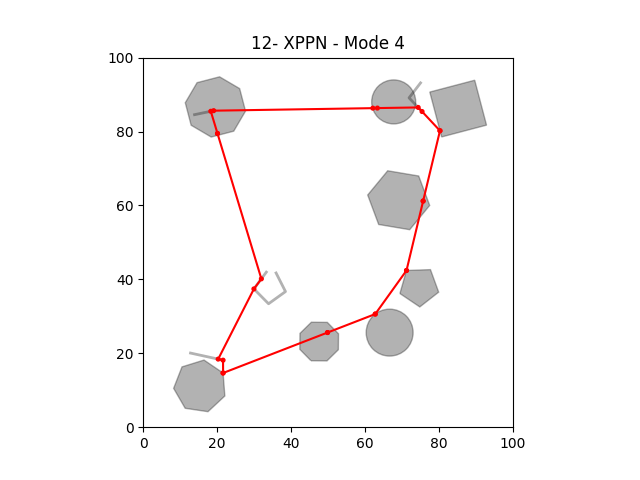
\includegraphics[width=1\linewidth]{example_xppn.png}
	    
	\end{frame}
	
	\begin{frame}{Example 2}
		
		\begin{center}
			\animategraphics[controls, width = 0.7\linewidth]{3}{gif_xppn/}{100}{1}
		\end{center}
	    
	\end{frame}
	
\end{document}
